\documentclass[11pt]{article}
\usepackage[utf8]{inputenc}
\usepackage[left=2cm,
            right=2cm,
            top=2.25cm,
            bottom=2.25cm,
            headheight=12pt,
            a4paper]{geometry}
\usepackage{amsmath}
\usepackage{amssymb}
\usepackage{amsfonts}
\usepackage{siunitx}
\usepackage{physics}
\usepackage{bm} % Bold-faced math
\usepackage{amsopn}
\usepackage[skip=10pt]{caption}
\usepackage{color}
\usepackage{xcolor,colortbl}
\usepackage[pdftex, bookmarks, colorlinks, breaklinks, allcolors=blue]{hyperref}
\usepackage{soul}
\hypersetup{colorlinks, citecolor=blue}
\usepackage[capitalise]{cleveref}
\usepackage{stmaryrd} % double brackets for jump operator
\usepackage{graphicx}


% Bibliography tools
\usepackage{csquotes}

% Set some length parameters
% \setlength{\parindent}{0pt}
% \setlength{\parskip}{10pt}
\setlength{\tabcolsep}{0.35cm}


%% Some new commands
% Partial derivatives
\newcommand{\pdifft}[1]{\frac{\partial  #1}{\partial t}}
\newcommand{\pdiffdifft}[1]{\frac{\partial^2 #1}{\partial t^2}}
\newcommand{\pdiffx}[1]{\frac{\partial #1}{\partial x}}
\newcommand{\pdiffy}[1]{\frac{\partial #1}{\partial y}}
\newcommand{\pdiffxi}[1]{\frac{\partial #1}{\partial x_i}}
\newcommand{\pdiffxj}[1]{\frac{\partial #1}{\partial x_j}}
\newcommand{\secpdiffx}[1]{\frac{\partial^2 #1}{\partial x^2}}
\newcommand{\secpdiffxi}[1]{\frac{\partial^2 #1}{\partial x_i \partial x_i}}
\newcommand{\secpdiffxj}[1]{\frac{\partial^2 #1}{\partial x_j \partial x_j}}

% Boundaries
\newcommand{\Schp}{\Gamma_{\mathrm{chp}}}

% Norms
\newcommand{\normltwo}[1]{{ \vert\vert#1\vert\vert}_{L^2}}
\newcommand{\normlinf}[1]{{\vert\vert#1\vert\vert}_{L^{\infty}}}
\newcommand{\Hnorm}[1]{\norm{#1}_{H^1}}
\newcommand{\Lnorm}[1]{\norm{#1}_{L^2}}

% Integrals
\newcommand{\intD}[1]{\int_{\mathcal{D}}#1 \, \mathrm{d}\bm{x}}
\newcommand{\intS}[1]{\int_{\mathcal{S}}#1 \, \mathrm{d}s}
\newcommand{\intE}[1]{\int_{\mathcal{E}}#1 \mathrm{d}S}
\newcommand{\intSs}[1]{\int_{\Gamma_s}#1 \, \mathrm{d}s}

% Discontinuity operators
\newcommand{\avg}[1]{\{#1\}}
\newcommand{\jump}[1]{\llbracket#1\rrbracket}

% Bold faced math characters
\newcommand{\ff}{\bm{f}}
\newcommand{\cc}{\bm{c}}
\newcommand{\nn}{\bm{n}}
\newcommand{\rr}{\bm{r}}
\newcommand{\uu}{\bm{u}}
\newcommand{\vv}{\bm{v}}
\newcommand{\ww}{\bm{w}}
\newcommand{\xx}{\bm{x}}
\newcommand{\yy}{\bm{y}}
\newcommand{\VV}{\bm{V}}
\newcommand{\TT}{\mathbb{T}}
\newcommand{\DD}{\mathcal{D}}
\newcommand{\Scal}{\mathcal{S}}
\newcommand{\bsigma}{\bm{\sigma}}
\newcommand{\bsigmahat}{\hat{\bm{\sigma}}}
\newcommand{\btau}{\bm{\tau}}
\newcommand{\beps}{\bm{\varepsilon}}
\newcommand{\bphi}{\bm{\phi}}

% Comments
\newcommand{\lyng}[1]{\textcolor{blue}{HH: #1}}
\newcommand{\fixme}[1]{\textcolor{red}{#1}}

\newcommand{\dx}{\, \mathrm{d}x}

\setcounter{footnote}{1}

% Title
\title{\textbf{Brain ventricular flow topology: a Lagrangian perspective}}
\author{
    H. Herlyng, S. Shadden
}

\date{\today}
% Optional PDF information
\ifpdf
\hypersetup{
  pdftitle={lagrangian-csf},
  pdfauthor={H.~Herlyng and S.~Shadden}
}
\fi

\begin{document}

\maketitle

\begin{abstract}
    This paper ...
\end{abstract}

\section{Introduction}
% I1: What is the problem - from big picture to our precise topic - why is it interesting?
Cerebrospinal fluid (CSF) flow is an important contributor to brain homeostasis
and the regulatory processes of the brain. Volume transmission is a theory that outlines
the importance of CSF flow in the neuromodulatory processes of the brain.

% I2: What do we know about the problem and the topic?
The underlying mechanisms of brain ventricular CSF flow have been studied extensively
in the last decades. Still a topic of debate, mounting evidence suggests that
the bulk pulsatile flow is associated with the cardiac and respiratory cycles.
Smaller flow scales are affected by beating of motile cilia lining the ventricular 
walls. Neural activity has also been shown to impact CSF flow patterns.
Simple visualizations of flow trajectories in animals have shown that
ventricular cerebrospinal fluid flow has intricate details,
with demonstrations of stagnation and separation points
and vortex-structured flows \cite{gilpin2017flowtrace,
Faubel2016CiliaVentricles,
Olstad2019CiliaryDevelopment}.
Lagrangian Coherent Structures (LCS) have proved themselves to be 
an informative way of studying advective transport in fluid flows
\cite{shadden2005definition, haller2015lagrangian}. Previous studies
have used LCS approximation to increase understanding of mixing 
and flow structures in blood flow~\cite{shadden2008characterization},
atmospheric flow~\cite{Gunther2021LagrangianWinds},
airway flow~\cite{lukens2010using},
oceanic flows, ... etc. 

% I3: What do we not know about the problem and what do we want to
% know? What are the precise research questions we want to address?
% Refer to specific studies and what specifically we do not know.
Flow and mixing mechanisms in the human central nervous system
and specifically the brain ventricles
are still not completely understood.
We want to study LCS in brain ventricles,
with the aim of gaining further
insights on flow and mixing in the ventricles, which impacts
CSF composition and thus neuromodulatory processes.

% I4: How do we address the problem and what do we find out?
In this work, we study intraventricular CSF flow in embryonic zebrafish and adult human brain ventricles.
The geometries are segmented from medical imaging data. First, we simulate CSF flow using a finite
element method. The CSF velocity fields are used to analyze flow topology using particle
trajectories and finite-time Lyapunov exponent fields.

\section{Methods}
\subsection{Finite-time Lyapunov exponent fields}
Consider the dynamical system
\begin{equation}
    \dot{\xx}(t; t_0, \xx_0) = \frac{\mathrm d\xx}{\mathrm d t} = \uu(\xx(t; t_0, \xx_0), t),
    \label{eq:dx_dt_equals_u}
\end{equation}
where $\xx(t)\in$ are the spatial coordinates of the domain $\mathcal{D}\subset\mathbb{R}^d$,
$t$ denotes time, $\uu$ is a velocity, and $\xx_0=\xx(t_0; t_0, \xx_0)$ is the initial
position at the initial time $t_0$. 
\Cref{eq:dx_dt_equals_u} can be integrated to yield the position at a time $T$:
\begin{equation}
    \xx(T) = \xx(t_0) + \int_{t_0}^T \uu(\xx, t)\,\mathrm d t.
\end{equation}
We define this relation as the mapping
\begin{equation}
    \bphi_{t_0}^t : \mathcal{D} \rightarrow \mathcal{D} : \xx_0 \mapsto \bphi_{t_0}^t(\xx_0) = \xx(t; t_0, \xx_0),
\end{equation}
where $\bphi_{t_0}^t$ is the flow map~\cite{shadden2005definition}.
We have thus far emphasized the dependence of 
the dynamical system and the flow map on the parameters $t_0, \xx_0$, but will in the 
following omit this notation for brevity. Using the gradient of the flow map,
we define the (right) Cauchy-Green deformation tensor
\begin{equation}
    \mathbf{C} = \left(\nabla\bphi_{t_0}^T\right)^*\nabla\bphi_{t_0}^T
\end{equation}
where $\mathbf{A}^*$ denotes the transpose of a tensor $\mathbf{A}$
and $T$ is the integration time. 
In the flow field $\uu(\xx, t)$, the maximum stretching that occurs between
two points $\xx$ and $\yy$ aligns with the eigenvector associated with
the maximum eigenvalue $\lambda_{\mathrm{max}}$ of $\mathbf{C}$~\cite{shadden2005definition}.
Related to this eigenvalue is the finite-time Lyapunov exponent, defined as
\begin{equation}
    \sigma_{t_0}^T(\xx) = \frac{1}{\vert T\vert}\log{\sqrt{\lambda_{\mathrm{max}}}}.
\end{equation}
With this definition, the maximum stretching of the flow can be formulated as
\begin{equation}
    \max||\delta\xx(\xx, t+t_0)|| = \exp\left(\sigma_{t_0}^T(\xx)|T|\right)||\overline{\delta\xx}(\xx, t_0)||,
\end{equation}
where $\overline{\delta\xx}(\xx, t_0)$ is the particle position change along
the eigenvector associated with $\lambda_{\mathrm{max}}$.
Note the absolute value of the integration time $T$,
which is employed because FTLE values can be calculated
both by integration forward ($T>0$) and backward ($T<0$) in time.
FTLE values associated with integration forward in time
reveal repelling structures (unstable manifolds),
whereas integration backward in time 
reveal attracting structures (stable manifolds).

\subsection{The governing equations of cerebrospinal fluid flow}
We consider flow of an incompressible, Newtonian fluid of density $\rho$ and dynamic viscosity
$\mu$ in a domain $\DD\subset\mathbb{R}^d$ with boundary $\partial\DD=\Scal$.
Neglecting the graviational force, no body forces are acting on the fluid.
The flow is governed by the Navier-Stokes equations,
in which the momentum equation reads
\begin{equation}
\rho\frac{D\uu}{\mathrm Dt}  = \rho\left(\pdifft{\uu} + (\uu\cdot\nabla)\uu\right) = \nabla\cdot\TT
\label{eq:momentum_navier_stokes}
\end{equation}
with the stress tensor $\TT$ defined as
\begin{equation*}
    \TT = 2\mu\beps(\uu) - p\mathbf{I},
\end{equation*}
where $\uu(\xx, t)$ and $p(\xx, t)$ are the fluid velocity and pressure,
$\mathbf{I}$ is the identity tensor in dimension $d$ and
$\beps(\uu)=\frac{1}{2}\left(\nabla\uu + (\nabla\uu)^T\right)$ is the
strain-rate tensor, or symmetric gradient, of $\uu$.
In addition to the momentum equation, the continuity equation
for an incompressible fluid reflects mass conservation:
\begin{equation}
    \nabla\cdot\uu = 0.
\end{equation}

The domain $\DD$ is deforming and varies over time. We therefore solve the Navier-Stokes
equations with an Arbitrary Eulerian Lagrangian (ALE) approach~\cite{Duarte2004ALE}.
The governing equations are solved in the reference configuration $\chi$,
using the mapping $\psi : \xx\mapsto\chi$ from the current deformed
configuration at time $t$ to the reference configuration.
In this setup, the governing equations are
\begin{alignat}{1}
    \rho\left(\pdifft{\uu} + ((\uu - \cc)\cdot\Tilde{\nabla})\uu\right) &= \Tilde{\nabla}\cdot\TT, \\
    \Tilde{\nabla}\cdot\uu &= 0,
\end{alignat}
where $\Tilde{\nabla}$ is the differential operator in the deformed domain.
The differential operators and integration measures of the weak formulation
are transformed appropriately to account for the domain motion~\cite{Scovazzi2007LectureNotes}.

We define the Reynolds number
\begin{equation*}
    \mathrm{Re} = \frac{\mathrm{inertial \ forces}}{\mathrm{viscous \ forces}} = \frac{\rho UL}{\mu},
\end{equation*}
where $U$ and $L$ are characteristic velocity and length scales, respectively.
In the human brain, flow measurements and simulations
indicate maximum Reynolds numbers in the
order of hundreds, meaning transient and inertial effects require
modeling by the Navier-Stokes equations~\cite{Gholampour2018FSI}.
In contrast, CSF flow in smaller brains, such as
embryonic zebrafish brain ventricles,
is dominated by viscous forces ($\mathrm{Re} \ll 1$)
\cite{Olstad2019CiliaryDevelopment, Herlyng2025AdvectionDiffusion}.
Consequently, the intertial terms (left-hand side of \Cref{eq:momentum_navier_stokes})
can be neglected, yielding the Stokes equations:
\begin{equation}
    - \nabla\cdot\TT = \bm{0}.
    \label{eq:stokes_eq}
\end{equation}

\subsection{Flow mechanisms and boundary conditions}
We consider three fluid motion-inducing mechanisms, and model them as follows:
\begin{itemize}
    \item Deformations of the brain ventricles related to the cardiac and respiratory cycles,
    modeled with an imposed deformation velocity
    \item Secretion of CSF from the choroid plexus,
    modeled with an influx boundary condition on the velocity
    \item Ciliary beating, modeled as a tangential traction acting on the fluid at the boundary
\end{itemize}
We impose zero normal traction at the lateral apertures and the cut-off of the spinal canal
to model them as open boundaries that allow for in- and outflow.

\subsubsection{Brain ventricles deformation}
To model ventricular wall deformations associated with the
cardiac and respiratory cycles, we impose a
deformation velocity as a boundary
condition when solving the flow equations.
This deformation velocity is obtained by
considering the brain ventricles as a
linear elastic solid and
modeling the deformation $\ww(\xx, t)$
of the ventricular walls through imposing
displacement boundary conditions.
The equations of linear elasticity can be written as
\begin{equation}
    \rho\pdiffdifft{\ww} - \nabla\cdot\bsigma_s = \bm{0} \quad\mathrm{in \ \mathcal{D}},
    \label{eq:strong_linear_elasticity_1}
\end{equation}
where $\bsigma_s = 2\eta\beps(\ww) + \lambda\mathrm{tr}(\beps(\ww))\delta$ is the
solid stress tensor, in which $\eta$ and $\lambda$ are the Lamé parameters of the ventricular walls
and $\delta$ is the Kronecker delta. Applying the divergence operator, \Cref{eq:strong_linear_elasticity_1}
takes the form
\begin{equation}
    \rho\pdiffdifft{\ww} - 2\eta\nabla\cdot\beps(\ww) - \lambda\nabla(\nabla\cdot\ww) = \bm{0},
    \quad\mathrm{in \ \mathcal{D}}.
\end{equation}
We impose the boundary conditions
\begin{align}
    \ww &= \bm{g} \quad\mathrm{on \ \mathcal{S}_1}, \\
    \bsigma_s\nn &= \bm{0} \quad\mathrm{on \ \mathcal{S}_2 = \mathcal{S}\setminus\mathcal{S}_1}.
\end{align}
On $\mathcal{S}_1$ we impose a given deformation $\bm{g}$, whereas
$\mathcal{S}_2$ is considered traction-free.
The displacement $\bm{g}$ is based on brain displacement
measurements~\cite{Kurtcuoglu2007ComputationalSylvius,
Enzmann1992BrainImaging} along the feet-head axis ($z$ axis),
and $\bm{g}$ therefore only has a $z$ component.
The Lamé parameters are derived from the Poisson's ratio $\nu=\fixme{0.35}$ and Young's modulus
$E=\fixme{350}$ Pa of white matter brain tissue that surrounds the ventricles
\cite{Cheng2010ComputationalModel, Cheng2007UnconfinedCompression}.

\subsubsection{Choroid plexus secretion}
CSF is mainly produced by the choroid plexus tissue.
We assume that all CSF that enters the brain ventricles
is produced by the choroid plexus, and that the influx is evenly distributed
over the production sites in the lateral, third and fourth ventricles.
However, in reality 10--30\% of the CSF production
may come from interstitial fluid transported through the ependymal cell
layer of the brain ventricles walls into the ventricles~\cite{Brodal2016TheSystem}.
The CSF secretion is modeled by imposing a normal flux at the
boundary $\Schp$ such that the total flux through the choroid plexus boundary is
\begin{equation}
    \int_{\Schp}(\uu\cdot\nn)\,\mathrm ds = Q.
\end{equation}
The total flux $Q=504$ ml/day is the daily total
CSF production in a human brain\cite{Czosnyka2004CerebrospinalDynamics}.

\subsubsection{Cilia forces}
Motile cilia are modeled by imposing forces on the fluid with a
boundary condition on the tangential traction
$P_{\nn}(\bsigmahat) = \btau = \tau P_{\nn}(\rr)$.
Here $\bsigmahat=\bsigma\nn$ is the traction vector and
$P_{\nn}(\cdot)$ is the projection of a vector onto a plane normal
to $\nn$. Work by Guirao \emph{et al.} indicates
that motile cilia beating direction is oriented by
CSF production during neural development~\cite{Guirao2010CouplingCilia}.
This was modeled by Siyahhan \emph{et al.}, who considered
directionality of the cilia forcing aligned
with the wall shear stress of the macroscopic flow simulated in a
production-only setup~\cite{Siyahhan2014FlowVentricles}.
We follow a similar approach, simulating CSF flow with the
boundary condition~\eqref{eq:choroid_plexus_BC} on $\Schp$,
a zero normal traction condition on the spinal canal and lateral apertures,
and $\uu\cdot\nn=0$ on the rest of the boundary. In the
tangential direction, the CSF is free to slip. The resulting velocity field,
$\uu_{\mathrm{prod}}$, is normalized in length to yield the direction of the cilia:
\begin{equation*}
    \rr = \frac{\uu_{\mathrm{prod}}}{|\uu_{\mathrm{prod}}|}.
\end{equation*}

The parameter $\tau$ determines the magnitude of $\btau$. In previous work on zebrafish modeling,
we determined $\tau$ heuristically by comparing simulated CSF velocity fields with in vivo
flow data~\cite{Olstad2019CiliaryDevelopment, Herlyng2025AdvectionDiffusion}.

Cilia directionality reference: Yamadori T.
The directions of ciliary beat on the wall of the fourth ventricle in the mouse.
Arch Histol Jpn 1977; 40: 283–296

\lyng{Should we do some "upper/lower bound" type of estimate?
E.g., in the "maximal force" setting, how much do cilia contribute to flow structures?}

\subsection{Numerical methods}
\subsubsection{Discretization}
We consider an $\bm{H}(\mathrm{div}; \DD)$-conforming discretization of 
the governing fluid equations using
Brezzi-Douglas-Marini (BDM) elements for the velocity and discontinuous Galerkin (DG)
elements for the pressure. The scheme conserves mass exactly pointwise.
This discretization ensures continuity in the velocity component normal
to facets. Tangential continuity is achieved by using the stabilization
outlined in Hong~\emph{et al.}~\cite{Hong2016AEquations}. A detailed derivation
of the discretization for the Stokes equations can be found in
Herlyng~\emph{et al.}~\cite{Herlyng2025AdvectionDiffusion}.

For the Navier-Stokes equations, the convective term
is linearized as
\begin{equation*}
    (\uu^{n+1}\cdot\nabla)\uu^{n+1} \approx (\uu^n\cdot\nabla)\uu^{n+1},
\end{equation*}
where $n$ denotes timestep. Convective fluxes both internal in the
mesh and on open boundaries are stabilized with
an upwinding technique~\cite{Schroeder2018Towards}.

Since we use an implicit time discretization, we only need an initial condition
for the velocity field and not the pressure.
When solving the Stokes equations, the fluid is considered being
initially at rest: $\uu_0(\xx)=\uu(\xx, 0)=\bm{0}$.
For the Navier-Stokes equations, we solve the Stokes equations and use the solution
$\uu_{\mathrm{Stk}}(\xx)$ as an initial condition;
$\uu_0(\xx)=\uu_{\mathrm{Stk}}(\xx)$. 

In time, we consider the implicit, second-order discretization scheme BDF2~\cite{Volker2016}.


\subsection{Ventricular geometries and model scenarios}
We consider two geometries: the ventricular geometry of an embryonic zebrafish at two days
post-fertilization (2 dpf), and the brain ventricles of an adult (healthy) human. In embryonic zebrafish,
choroid plexus secretion begins at a later developmental stage than 2 dpf. Therefore, we only consider
cilia forces in this flow model, and the domain is closed.
For the human brain, we impose both deformation, choroid plexus
secretion and cilia forces, and the lateral apertures and the spinal canal are open boundaries.

\section{Results}
\subsection{Finite element flow simulations}
We present the CSF flow simulated in the brain ventricles. 
\begin{figure}
    \centering
    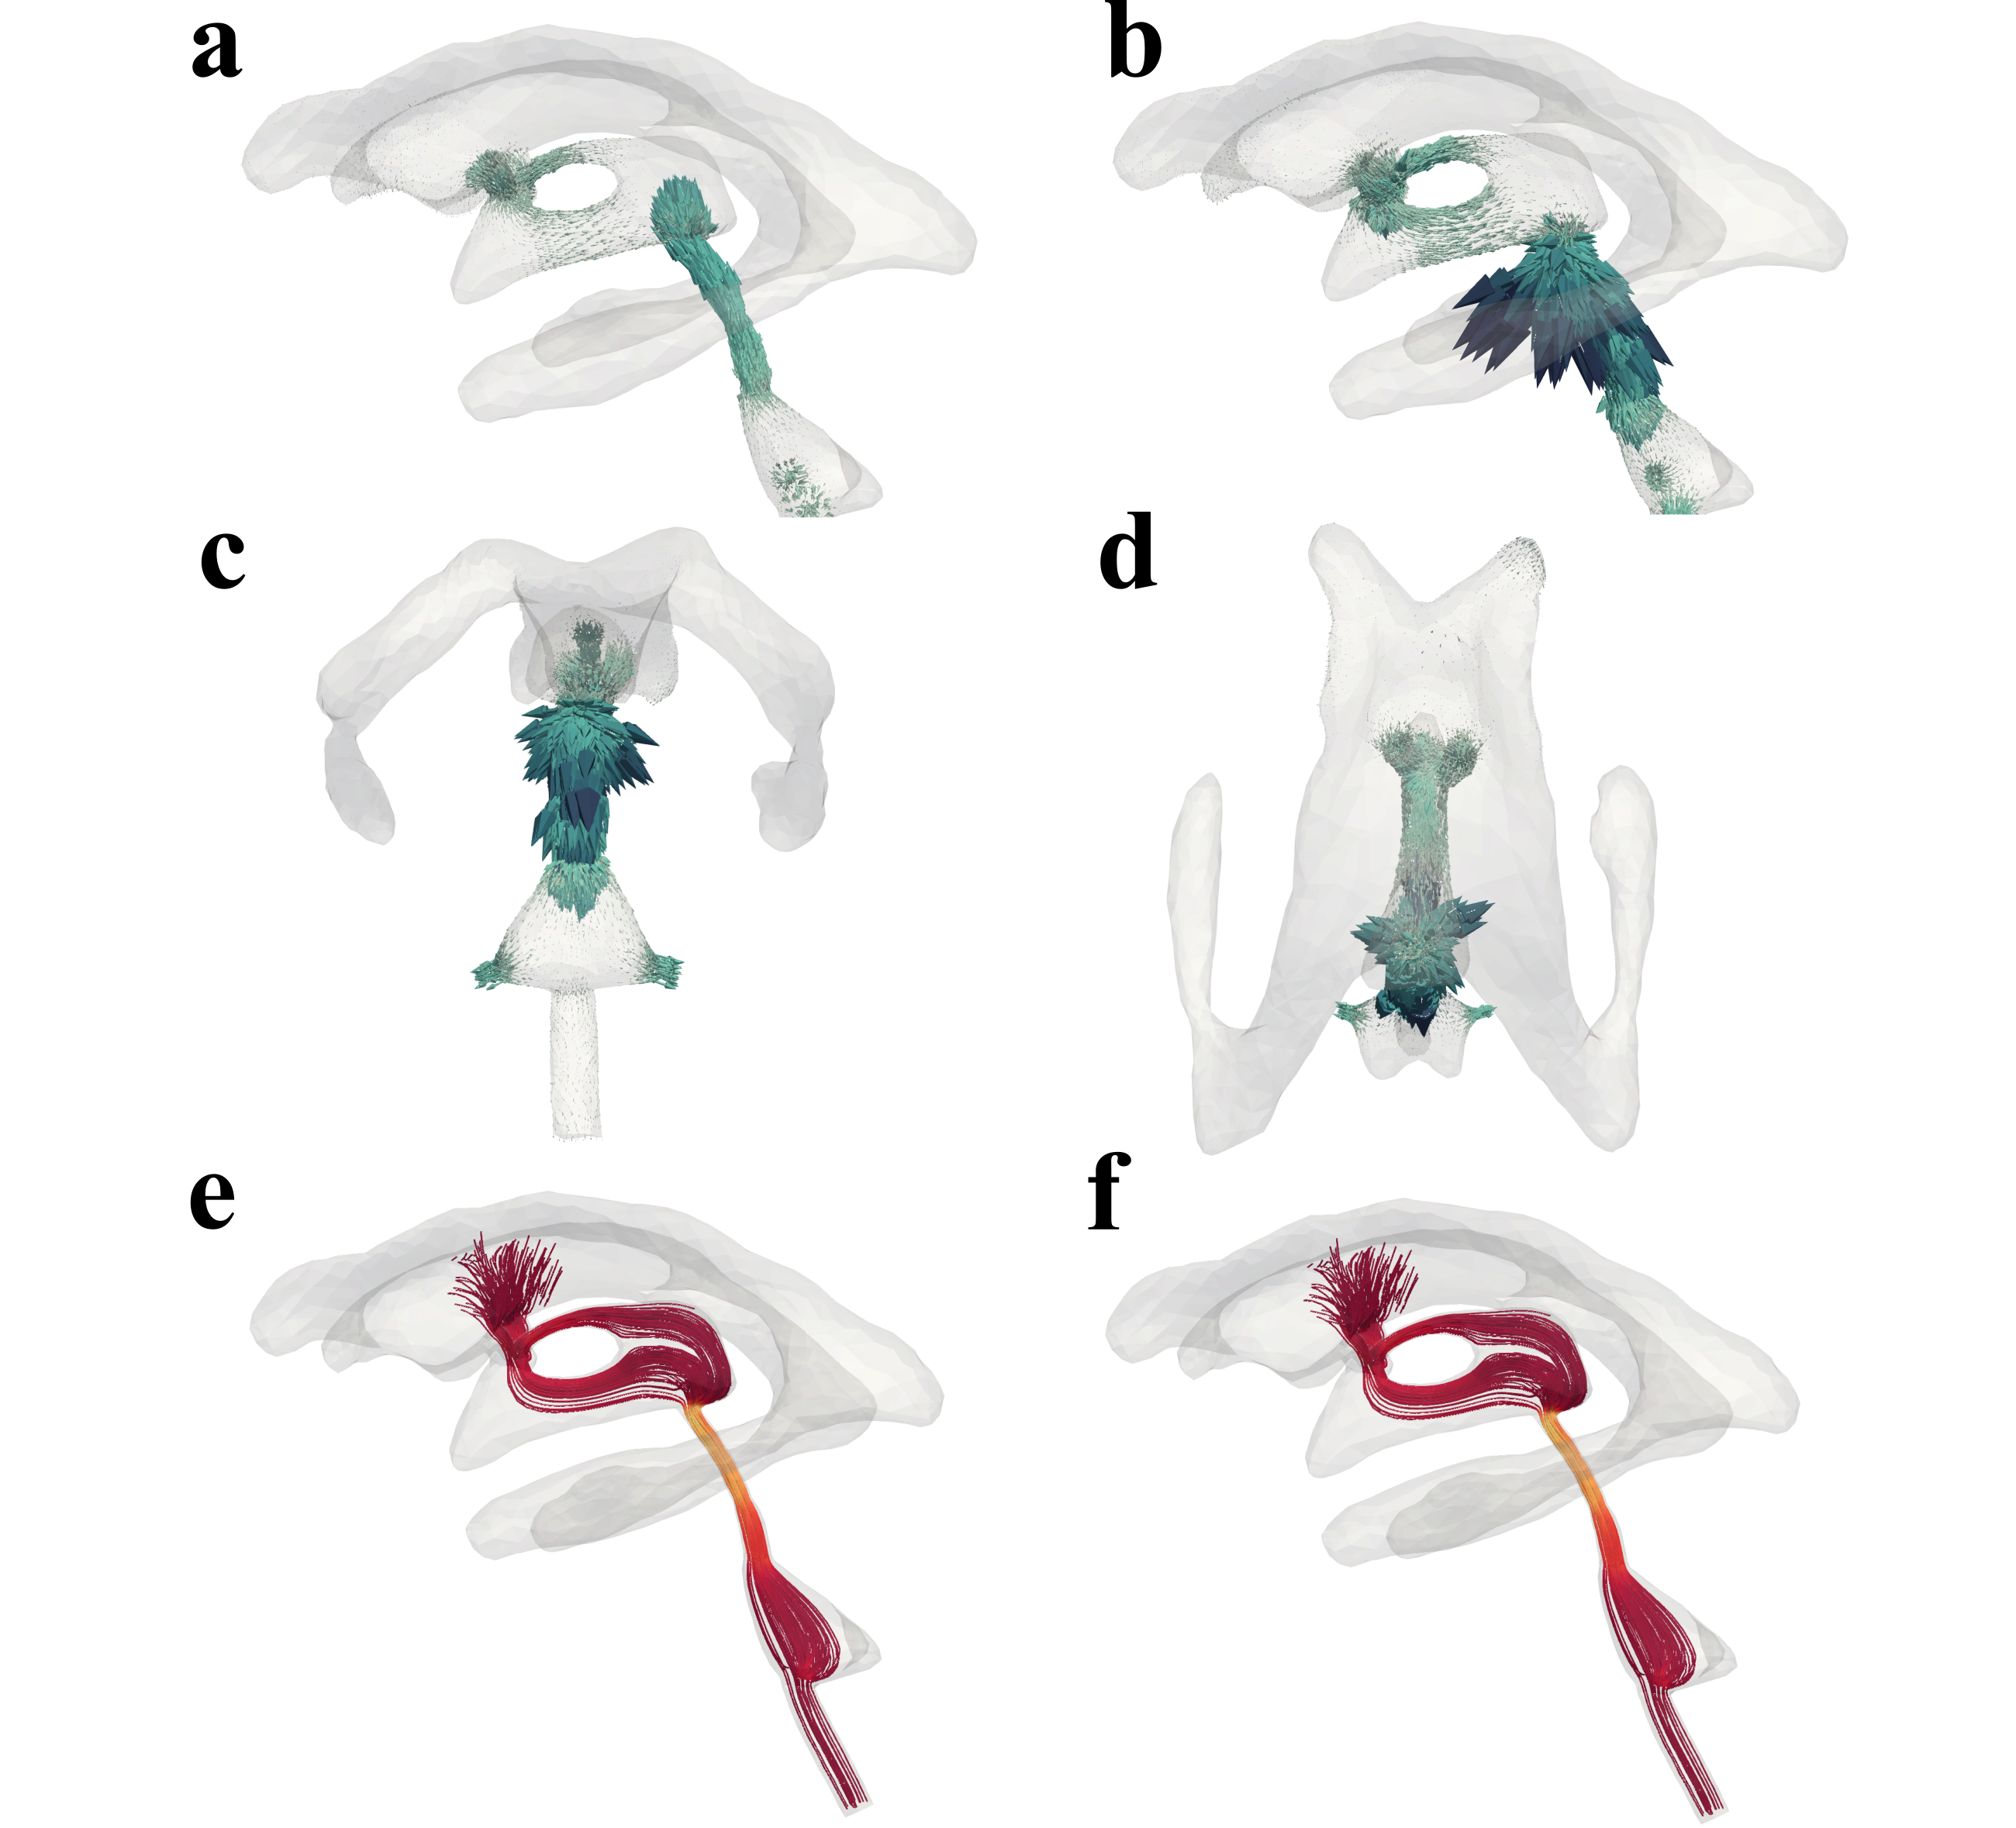
\includegraphics[width=\textwidth]{graphics/figure1.png}
    \caption{Caption.}
    \label{fig:fig1}
\end{figure}

\subsection{FTLE fields demonstrate ventricular flow compartmentalization in zebrafish embryos}
We present FTLE fields for the different brains in. The forward (repelling)
and backward (attracting) structures in the
anterior-middle interventricular duct in the zebrafish
brain ventricles combine to generate a separatrix.
This separatrix is structured such that flow is
compartmentalized in the anterior and middle ventricles.
These results align well with previous studies that have
demonstrated flow compartmentalization in embryonic zebrafish
brain ventricles~\cite{Olstad2019CiliaryDevelopment, Herlyng2025AdvectionDiffusion}.
\begin{figure}
    \centering
    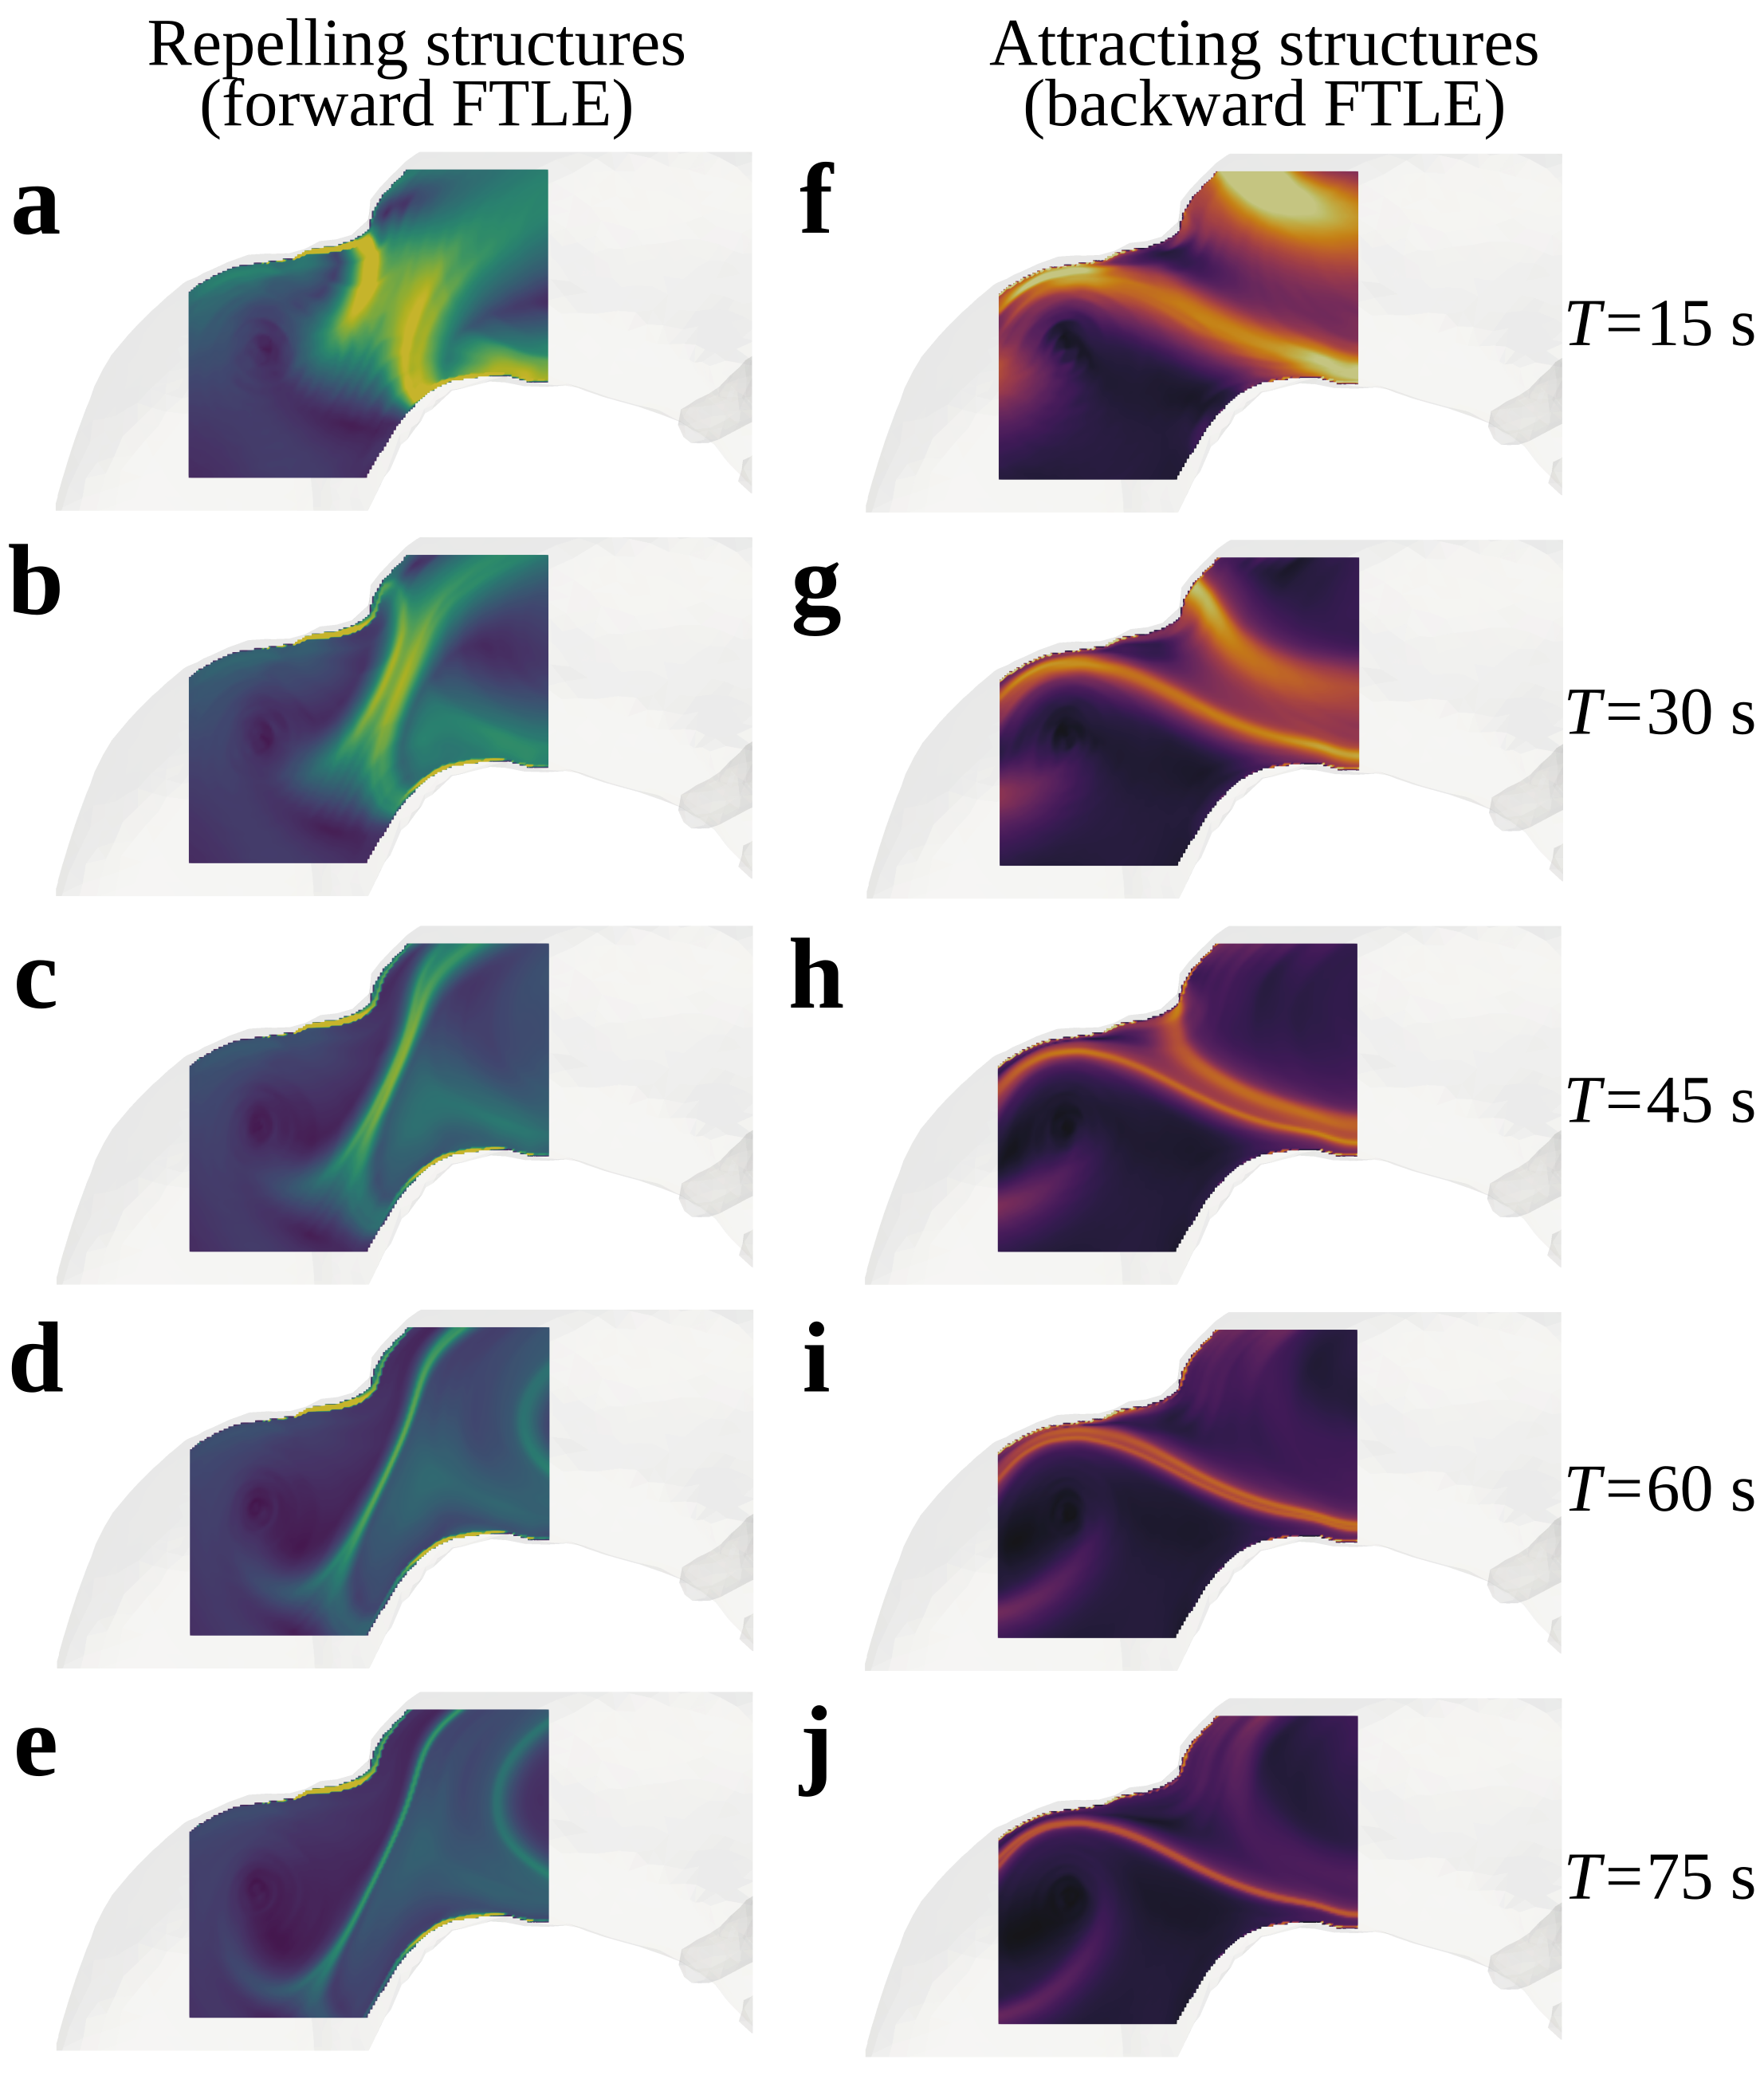
\includegraphics[width=\textwidth]{graphics/figure2.png}
    \caption{Caption.}
    \label{fig:fig2}
\end{figure}

\section{Verification and validation}
Convergence properties of the discretization scheme were assessed with two
model problems. To assess spatial convergence, we solved a channel flow
problem, observing linear convergence in both the velocity error measured
in the $\bm{H}^1$ semi-norm and the pressure error measured in the $L^2$ norm.
Temporal convergence was assessed
with a Taylor vortex problem~\cite{Karniadakis2005Verification},
where the second-order accuracy of the BDF2 scheme was confirmed.

To assess the physiological validity of the flow, we compare some
quantities of interest with previous works
\cite{Kurtcuoglu2007ComputationalSylvius,
Causemann2022HumanFramework,
Vinje2019RespiratoryMeasurements}:
\begin{itemize}
    \item The pressure gradient in the cerebral aqueduct

    \item The flow rate in the cerebral aqueduct and the outlet to the spinal canal
\end{itemize}

\clearpage

\bibliography{references}{}
\bibliographystyle{unsrturl}



% \subsection{Weak formulations}
% In deriving weak formulations of the Navier-Stokes and the Stokes equations,
% we will use the function spaces
% \begin{alignat*}{2}
%     Q &= L^2_0(\mathcal{D}) &&= \bigg\{q \ : \ \int_{\mathcal{D}}q^2 \dx < \infty, \ \int_{\mathcal{D}}q\dx = 0\bigg\}, \\
%     \VV &= \bm{H}^1(\mathcal{D}) &&= \bigg\{\vv \ : \ \vv\in\bm{L}^2, \
%     \int_{\mathcal{D}}\nabla\vv : \nabla\vv \dx < \infty\bigg\},
% \end{alignat*}
% where a bold-faced function space denotes a $d$-dimensional vector space,
% e.g. $\bm{H}^1 = [H^1]^d$. 

% \subsubsection{Stokes equations}
% We will first consider a weak form
% of the Stokes equations (\Cref{eq:stokes_eq}). We only briefly
% present the derivation, as it is similar to the one presented
% in detail in the appendix of
% Herlyng~\emph{et al.}~\cite{Herlyng2025AdvectionDiffusion}.
% The boundary $\partial\DD = \Scal = \Scal_1\cup\Scal_2\cup\Scal_3$
% is split into three parts: on $\Scal_1$ the deformation
% velocity $\dot{\ww}$ is imposed in the normal direction;
% on $\Scal_2$ the
% production boundary condition $Q$ is imposed in the normal direction;
% on $\Scal_3$ a zero normal traction is imposed. On both $\Scal_1$ and
% $\Scal_2$ cilia tangential traction is imposed in the tangential
% direction.
% Let the velocity $\uu\in\VV$ and the pressure
% $p\in Q$. Multiplying \Cref{eq:stokes_eq} by a test
% function $\vv\in\VV$, integrating over the domain $\mathcal{D}$,
% and integrating by parts, we have
% \begin{equation*}
%     \intD{\TT\nn\cdot\vv} = \bm{0}, \forall\vv\in\VV.
% \end{equation*}
% Inserting $\TT = 2\mu\beps(\uu) - p\mathbf{I}$ with
% $\beps(\uu)=\frac{1}{2}\left(\nabla\uu + (\nabla\uu)^T\right)$
% we have
% \begin{equation*}
%     \intD{(2\mu\beps(\uu) - p\mathbf{I})\nn\cdot\vv} =
%     \intD{(\mu\left(\nabla\uu + (\nabla\uu)^T\right) - p\mathbf{I})\nn\cdot\vv} = \bm{0}, \forall\vv\in\VV.
% \end{equation*}


% \subsubsection{Navier-Stokes equations}
% We will now derive a
% weak formulation of the Navier-Stokes equations. 
% Multiplying the momentum equation
% (\Cref{eq:momentum_navier_stokes}) with a 
% test function $\vv\in\VV$, integrating over
% the domain $\mathcal{D}$, and integrating the stress term
% by parts, we have
% \begin{equation*}
%     \intD{\rho\left(\pdifft{\uu}
%     + (\uu\cdot\nabla)\uu\right)\cdot\vv}
%     - \intS{\TT\nn\cdot\vv}
%     + \intD{\TT:\nabla\vv} = 0.
% \end{equation*}


% The discretization considered here is based on the work by Hong~\emph{et al.}~\cite{Hong2016AEquations}. We let the subscript $h$ denote discretized variables. Consider~\eqref{eq:stokes_weak_form_abstract} with discrete variables:
% \begin{subequations}
% \begin{alignat}{2}
%     a(\uu_h, \vv_h) + b(p_h, \vv_h) &= L(\vv_h), &&\quad\forall\vv_h\in\VV_h, \\
%     b(q_h, \uu_h) &= 0, &&\quad\forall \: q_h\in Q_h,
% \end{alignat}
% \label{eq:stokes_weak_form_discrete}%
% \end{subequations}%
% with the discrete function spaces $\VV_h$ and $Q_h$.
% Discretizing the variables in~\eqref{eq:stokes_weak_form_discrete} with $\mathrm{BDM}_k-\mathrm{DG}_{k-1}$ elements, this is not automatically stable discretization. To ensure coercivity and continuity of the bilinear form, we need to add the following stabilization terms to the weak form:
% \begin{equation}
%     \begin{aligned}
%       a_{\mathrm{stab}}(\uu_h, \vv_h) = &-\intE{\avg{2\mu\bm{\varepsilon}(\uu_h)\nn}\cdot\jump{P_{\nn}(\vv_h)}} \\
%                                                 &-\intE{\avg{2\mu\bm{\varepsilon}(\vv_h)\nn}\cdot\jump{P_{\nn}(\uu_h)}} \\
%                                                 &+2\mu\frac{\gamma}{h_a}\intE{\jump{P_{\nn}(\uu_h)}\cdot\jump{P_{\nn}(\vv_h)}}, \\
%     \end{aligned}
% \end{equation}
% where $\mathcal{E}$ are all internal facets of the mesh. Furthermore,
% $\gamma > 0$ is a penalty parameter which must be chosen large enough and
% $h_a$ is the average cell diameter of two neighboring elements.
% The jump and average operators $[[\cdot]]$ and $\{\cdot\}$ of a variable $\bm{\phi}$ are defined as
% \begin{align}
%     \jump{\bm{\phi}} &= \bm{\phi}\vert_{+} - \bm{\phi}\vert_{-}, \\
%     \avg{\bm{\phi}}  &= \frac{1}{2}\big((\bm{\phi}\cdot\nn)\vert_{+} - (\bm{\phi}\cdot\nn)\vert_{-} \big),
% \end{align}
% where $\bm{\phi}\vert_{+}$ is used to denote the value of the variable $\bm{\phi}$ on the side of the edge $\mathcal{E}$ where $\nn$ is pointing out of the cell. Correspondingly, $\bm{\phi}\vert_{-}$ is the variable value on the side of the edge $\mathcal{E}$ where  $\nn$ is pointing inwards.



\end{document}